\documentclass{article}

\usepackage{tikz}
\usetikzlibrary{calc}
\usetikzlibrary{positioning}

\usepackage{amssymb}


% Now we define the global styles

% We start by defining the default colours of vertices, edges and faces
\newcommand{\vertexColor}{blue}
\newcommand{\edgeColor}{black}
\newcommand{\faceColor}{yellow}

\newcommand{\vSize}{2.5pt}    % How big are the vertex circles (if drawn)?
% Command to set the vertex labels (in the correct colour)

\newcommand{\drawEdge}[3]{            
	\node[edgeBackground] at ($1/2*(#1)+1/2*(#2)$) {#3};
}


\tikzset{vertex/.style = {\vertexColor}}
\tikzset{edge/.style = {\edgeColor, thick}}
\tikzset{edgeBackground/.style = {fill=blue!20!white}}
\tikzset{face/.style = {fill=\faceColor, draw=\edgeColor}}


\begin{document}

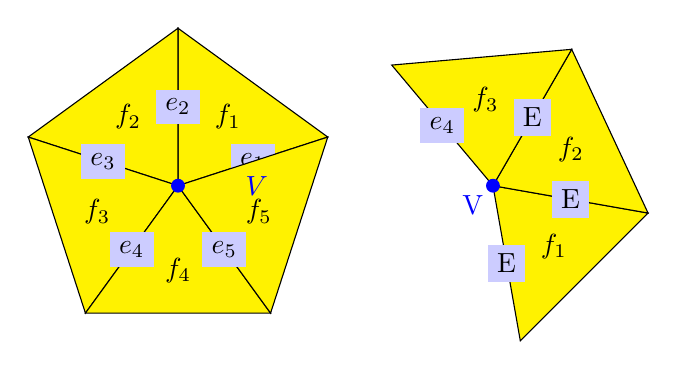
\begin{tikzpicture}
                        \def\r{2}
                        
                        \begin{scope}
                            \coordinate (A) at (0,0);
                            \coordinate (B1) at (18:\r);
                            \coordinate (B2) at (90:\r);
                            \coordinate (B3) at (162:\r);
                            \coordinate (B4) at (234:\r);
                            \coordinate (B5) at (306:\r);

                            \foreach \p/\q/\F/\E in {B1/B2/$f_1$/$e_1$, 
                                    B2/B3/$f_2$/$e_2$, B3/B4/$f_3$/$e_3$, 
                                    B4/B5/$f_4$/$e_4$, B5/B1/$f_5$/$e_5$}
                            {
                                \filldraw[face] (A) -- (\p) -- (\q) -- cycle;
                                \node at ($1/3*(A)+1/3*(\p)+1/3*(\q)$) {\F};
                                \drawEdge{A}{\p}{\E}
                            }

                            \fill[vertex] (A) circle (\vSize);
                            \node[vertex,right of=A] {$V$}; 
                        \end{scope}

                        \begin{scope}[xshift=4cm]
                            \def\w{70}
                            \def\start{-80}
                            \coordinate[label={[vertex]below left:V}] (A) at (0,0);
                            \coordinate (B1) at (\start:\r);
                            \coordinate (B2) at (\start+\w:\r);
                            \coordinate (B3) at (\start+2*\w:\r);
                            \coordinate (B4) at (\start+3*\w:\r);

                            \foreach \p/\q/\F/\E in {B1/B2/$f_1$/$e_1$,
                                    B2/B3/$f_2$/$e_2$, B3/B4/$f_3$/$e_3$}
                            {
                                \filldraw[face] (A) -- (\p) -- (\q) -- cycle;
                                \node at ($1/3*(A)+1/3*(\p)+1/3*(\q)$) {\F};
                                \drawEdge{A}{\p}{E}
                            }
                            
                            \drawEdge{A}{B4}{$e_4$};
                            \fill[vertex] (A) circle (\vSize);
                        \end{scope}
                    \end{tikzpicture}

\end{document} 